\documentclass[tikz,border=2mm]{standalone}

\begin{document}

\tikzset{every picture/.style={line width=0.75pt}} %set default line width to 0.75pt

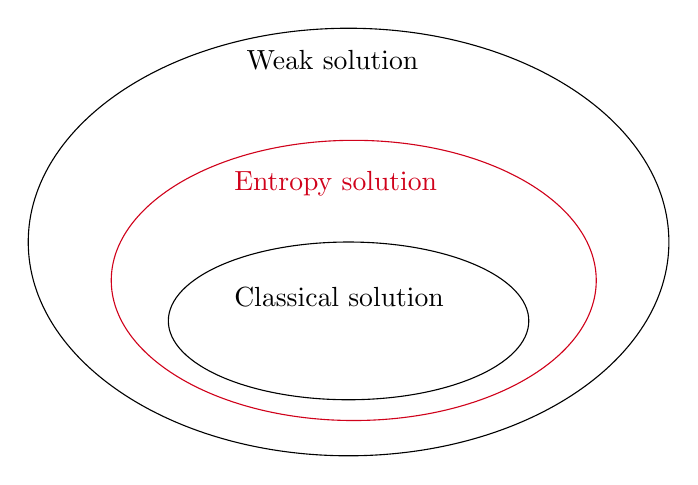
\begin{tikzpicture}[x=0.75pt,y=0.75pt,yscale=-1,xscale=1]
    %uncomment if require: \path (0,346); %set diagram left start at 0, and has height of 346

    %Shape: Ellipse [id:dp49241408905173856]
    \draw   (112,162.49) .. controls (112,105.6) and (181.1,59.49) .. (266.33,59.49) .. controls (351.57,59.49) and (420.67,105.6) .. (420.67,162.49) .. controls (420.67,219.37) and (351.57,265.49) .. (266.33,265.49) .. controls (181.1,265.49) and (112,219.37) .. (112,162.49) -- cycle ;
    %Shape: Ellipse [id:dp3689129779708782]
    \draw  [color={rgb, 255:red, 208; green, 2; blue, 27 }  ,draw opacity=1 ] (152,180.99) .. controls (152,143.71) and (204.31,113.49) .. (268.83,113.49) .. controls (333.36,113.49) and (385.67,143.71) .. (385.67,180.99) .. controls (385.67,218.27) and (333.36,248.49) .. (268.83,248.49) .. controls (204.31,248.49) and (152,218.27) .. (152,180.99) -- cycle ;
    %Shape: Ellipse [id:dp1544161738383112]
    \draw   (179.5,200.49) .. controls (179.5,179.5) and (218.38,162.49) .. (266.33,162.49) .. controls (314.29,162.49) and (353.17,179.5) .. (353.17,200.49) .. controls (353.17,221.48) and (314.29,238.49) .. (266.33,238.49) .. controls (218.38,238.49) and (179.5,221.48) .. (179.5,200.49) -- cycle ;

    % Text Node
    \draw (216,69) node [anchor=north west][inner sep=0.75pt]   [align=left] {Weak solution};
    % Text Node
    \draw (210,127) node [anchor=north west][inner sep=0.75pt]  [color={rgb, 255:red, 208; green, 2; blue, 27 }  ,opacity=1 ] [align=left] {Entropy solution};
    % Text Node
    \draw (210,183) node [anchor=north west][inner sep=0.75pt]   [align=left] {Classical solution};


\end{tikzpicture}

\end{document}
